\documentclass{article}
\usepackage{geometry}
\usepackage{graphicx}
\usepackage{enumitem}

\geometry{a4paper, left=1in, right=1in, top=1in, bottom=1in}

\title{Micro-benchmarks: A comparison of C++, Rust, and Zig}
\author{Fucă Răzvan-Ionuț \\ Technical University of Cluj-Napoca}

\date{}

\begin{document}
\maketitle
\vspace*{\fill}

\clearpage
\tableofcontents
\clearpage

\section{Introduction}
\subsection{Context}
The purpose of this project is to conduct a comprehensive benchmark of the execution time of various processes in three distinct programming languages: C++, Rust, and Zig. These languages have been chosen due to their classification as "systems programming languages," which means they offer direct access to hardware while also providing a robust, OS-agnostic API. Notably, they all support multi-threading, making them suitable for low-level and high-performance tasks. This project will delve into the nuances of these languages, shedding light on their capabilities and performance characteristics.

\subsection{Language selection}
The languages chosen for this project are:
\begin{itemize}
    \item C++ - A widely used systems programming language that offers extensive control over memory management and hardware interactions. C++ has a long history and a rich ecosystem of libraries and tools.
    \item Rust - A modern systems programming language known for its strong focus on memory safety without sacrificing performance. Rust's unique ownership system and borrowing rules set it apart from traditional languages.
    \item Zig - An up-and-coming systems programming language that combines a C-like syntax with modern features and a focus on compile-time safety. Zig's custom allocators and comptime code are key features that distinguish it.
\end{itemize}

\subsection{Objectives}
The primary objectives of this project are:
\begin{itemize}
    \item Develop sample programs in each of the selected languages that are specifically designed to test the performance of critical processes, including:
    \begin{itemize}
        \item Memory allocation
        \item Static memory access
        \item Dynamic memory access
        \item Thread creation
        \item Thread context switch
        \item Thread migration
    \end{itemize}
    \item Execute the sample programs in order to collect and interpret the data.
\end{itemize}

\subsection{Hypothesis}
The hypothesis for this project is that the results of the benchmarks will demonstrate close performance characteristics among the selected languages. This expectation is based on the fact that all three languages ultimately compile down to assembly instructions, but differences will arise from:
\begin{itemize}
    \item Compiler Optimizations: Each language's compiler applies its own set of optimizations, affecting execution speed.
    \item Programming Paradigms: The choice of language influences the programming paradigms and patterns used, which can impact performance.
    \item Memory Management Strategies: The languages vary in their approach to memory management, such as C++ relying on manual memory management, Rust utilizing its borrow checker, and Zig offering custom allocators.
\end{itemize}
\clearpage

\section{Bibliographic Study}
\subsection{Introduction to the languages}
The programming languages selected for this micro-benchmarking study are C++, Rust, and Zig. These languages have the ability to provide low-level control over hardware resources and memory management. In this section, we provide an overview of these languages and their relevance to our benchmarking project.
\begin{itemize}
    \item C++ is a well-established systems programming language known for its versatility and extensive control over memory management and hardware interactions. It has a rich history, starting as an extension of C in 1979.
    \item Rust is a modern systems programming language that has garnered attention for its emphasis on memory safety without compromising performance. It distinguishes itself with its ownership system and borrowing rules, forcing the programmer to adopt the RAII (resource acquisition is initialization) programming pattern, eliminating common sources of memory-related bugs.
    \item Zig is an emerging systems programming language that combines a C-like syntax with modern features. It places a strong focus on compile-time safety, which aligns well with our objective to assess language-level safety and performance. Notably, Zig offers features like custom allocators and compile-time code that set it apart from traditional systems programming languages.
\end{itemize}

\subsection{Visualization tools}
To effectively present and analyze the data collected from our benchmarking programs, we will utilize Matplotlib, a widely-used Python library for creating high-quality data visualizations. Matplotlib provides a versatile and user-friendly platform for generating graphs and charts, making it an ideal choice for representing the performance metrics obtained during our micro-benchmarking study. Matplotlib has also been chosen because of its ease of processing external data such as CSV files.
\clearpage

\section{Analysis \& Design}
The programs will be CLI apps obeying *NIX philosophy that will perform a series of algorithms designed to benchmark the aforementioned processes and will dump the results to a file in a plot-friendly format (CSV) that will later be processed by a script that will prune and interpret the data.
Figure \ref{fig:flow} showcases the general flow of data in our project.
\begin{figure}[h]
    \centering
    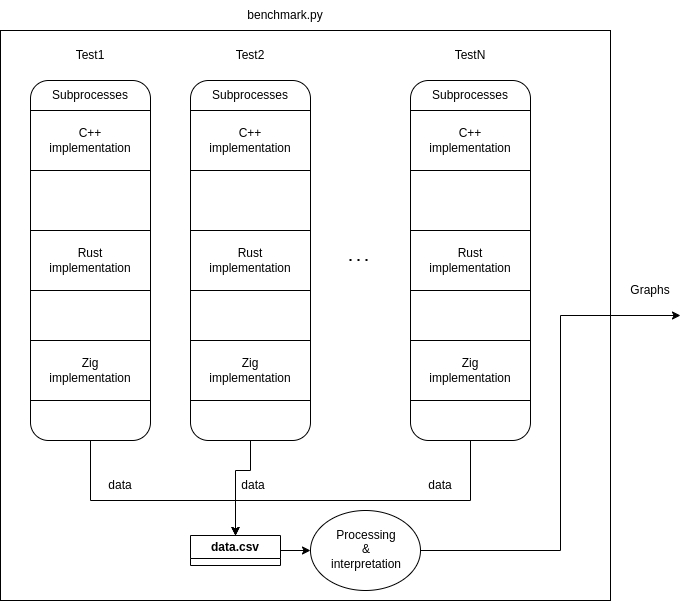
\includegraphics[width=0.8\textwidth]{structure.png}
    \caption{General flow of data in the project.}
    \label{fig:flow}
\end{figure}


The type of benchmarks that will be performed can be grouped quite easily into two main categories:
\begin{itemize}
    \item Memory benchmarks
    \item Threading benchmarks
\end{itemize}

\subsection{Memory benchmarks}
For the memory benchmarks, the programs will perform a series elementary operations on increasingly larger common data structures. A complete list of actions to be performed that I believe will encompass most common applications is:
\begin{itemize}
    \item Allocating dynamic arrays
    \item Creating linked lists (or similar dynamic data structures)
    \item Performing operations such as sorting or traversals on the created data structures
\end{itemize}

\subsection{Threading benchmarks}
For the threading benchmarks, the measuring process will be a little more difficult as there is no explicit way of directly accomplishing our desired results; however, there are workarounds that will force the OS to perform operations such as context switching and migration. A list of actions that I believe will adequately measure the desired processes consists of:
\begin{itemize}
    \item Calling an empty function in a synchronous and asynchronous way and computing the difference between the two to gather quantitative data regarding thread creation
    \item Writing and reading bytes of data from a pipe to force two thread context switches
    \item Setting thread CPU affinity using functions like \texttt{pthread\_set\_affinity\_np} or similar depending on the platform to force thread migration
\end{itemize}

All of these benchmarks will be time-based, using each of the language's built-in time measuring method that will yeild results in nanoseconds:
\begin{itemize}
    \item C++ \texttt{std::chrono::high\_resolution\_clock}
    \item Zig's \texttt{std.time.Timer}
    \item Rust's \texttt{std::time::Instant}
\end{itemize}

\clearpage
\section{Implementation}
\subsection{Memory tests, dynamic data}
The first step of running our benchmarks is implementing the necessary data structures we need to test. The most notable of the data structures is a generic singly linked list that will showcase each language's lower-level features (manual memory allocation, the use of pointers and nullable/optional data types, etc.), as well as higher-level features (OOP, static and dynamic dispatch, or compile-time code), and the programming paradigm they encourage.

The implementation details of each are described below:
\begin{itemize}
    \item \textbf{C++} – Singly linked list using templates
    \item \textbf{Zig} – Compile-time function that returns a new type
    \item \textbf{Rust} – Generic list that uses the 'Box' smart pointer for dynamic memory allocation
\end{itemize}

Another test relies on the dynamic allocation of large arrays on the heap using each of the languages specific constructs
\begin{itemize}
    \item \textbf{C++} – Using the new operator
    \item \textbf{Zig} – Using different allocators provided by the standard library
    \item \textbf{Rust} – Using Vec::with\_capacity as it is the closest analogue to allocating a dynamic array of a known size in rust
\end{itemize}

\subsection{Memory tests, static data}

Each program will allocate an array on the stack of size 100000 and then traverse it, setting the value of each entry in the array to their index.

\subsection{Threading tests, thread creation}

Each program will run a function that returns as soon as possible. At first by launching it in a thread, and secondly by running it directly.
We will measure the time difference between these two scenarios in order to quantify thread creation.

This will be accomplished using:
\begin{itemize}
    \item \textbf{C++} – std::thread
    \item \textbf{Zig} – std.Thread
    \item \textbf{Rust} - std::thread
\end{itemize}

\subsection{Threading tests, thread context switch}
The programs will create a child thread and ping\_pong a single byte between parent and child. This will force two thread context switches per read/write
\subsection{Threading tests, thread migration}
The programs will leverage pthread\_set\_affinity\_np in order to force the tested thread to run on a single particular processor. We will force the thread to migrate from processor one to processor two using the linux system call sched\_yield.

\subsection{Benchmarking script}
The script that will run and aggregate the data generated by the programs is benchmark.py. This benchmarking script relies on a couple of files 
\begin{itemize}
    \item \textbf{config.yaml} Where the benchmarks parameters will be defined. Ex (Size of array, number of runs, weather or not to recompile the programs) etc.
    \item \textbf{data.csv} where all the programs will dump their results
\end{itemize}
The script also provides a GUI in if the user prefers to use it instead of a config file.

\clearpage
\section{Bibliography}
\begin{enumerate}
    \item \textit{C++ language reference}. [Online]. Available: \texttt{https://en.cppreference.com/w/cpp/language}
    \item \textit{Rust language reference}. [Online]. Available: \texttt{https://doc.rust-lang.org/stable/reference/}
    \item \textit{Zig language reference}. [Online]. Available: \texttt{https://ziglang.org/documentation/master/}
    \item \textit{Matplotlib documentation}. [Online]. Available: \texttt{https://matplotlib.org/stable/index.html}
    \item \textit{Rust by example: RAII}. [Online]. Available: \texttt{https://doc.rust-lang.org/rust-by-example/scope/raii.html}
\end{enumerate}

\end{document}
